\begin{figure}
    \centering
    \begin{subfigure}{0.24\linewidth}
        \centering
        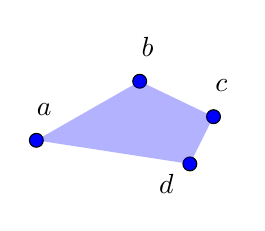
\begin{tikzpicture}
            \node[draw, circle, black, fill=blue, inner sep=0pt, minimum size=5pt, label={[xshift=0.1cm, yshift=0.1cm]$a$}] (a) at (0*0.75,0*0.75) {};
            \node[draw, circle, black, fill=blue, inner sep=0pt, minimum size=5pt, label={[xshift=0.1cm, yshift=0.1cm]$b$}] (b) at (1.75*0.75,1*0.75) {};
            \node[draw, circle, black, fill=blue, inner sep=0pt, minimum size=5pt, label={[xshift=0.1cm, yshift=0.1cm]$c$}] (c) at (3*0.75,0.4*0.75) {};
            \node[draw, circle, black, fill=blue, inner sep=0pt, minimum size=5pt, label={[xshift=-0.3cm, yshift=-0.6cm]$d$}] (d) at (2.6*0.75,-0.4*0.75) {};
            \coordinate (a) at (0*0.75,0*0.75);
            \coordinate (b) at (1.75*0.75,1*0.75);
            \coordinate (c) at (3*0.75,0.4*0.75);
            \coordinate (d) at (2.6*0.75,-0.4*0.75);
            \fill[blue, opacity=0.3] (a) -- (b) -- (c) -- (d) -- (a) -- cycle;
        \end{tikzpicture}
        \caption{}\label{fig:equiv-a}
    \end{subfigure}
    \begin{subfigure}{0.24\linewidth}
        \centering
        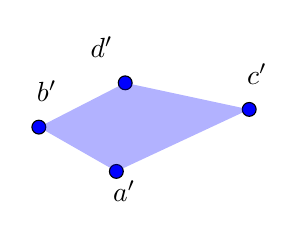
\begin{tikzpicture}[scale=0.75]
            \node[draw, circle, black, fill=blue, inner sep=0pt, minimum size=5pt, label={[xshift=0.1cm, yshift=-0.6cm]$a'$}] (a) at (0*0.75,0*0.75) {};
            \node[draw, circle, black, fill=blue, inner sep=0pt, minimum size=5pt, label={[xshift=0.1cm, yshift=0.1cm]$b'$}] (b) at (-1.75*0.75,1*0.75) {};
            \node[draw, circle, black, fill=blue, inner sep=0pt, minimum size=5pt, label={[xshift=0.1cm, yshift=0.1cm]$c'$}] (c) at (3*0.75,1.4*0.75) {};
            \node[draw, circle, black, fill=blue, inner sep=0pt, minimum size=5pt, label={[xshift=-0.3cm, yshift=0.1cm]$d'$}] (d) at (0.2*0.75,2*0.75) {};
            \coordinate (a) at (0*0.75,0*0.75);
            \coordinate (b) at (-1.75*0.75,1*0.75);
            \coordinate (c) at (3*0.75,1.4*0.75);
            \coordinate (d) at (0.2*0.75,2*0.75);*0.75
            \fill[blue, opacity=0.3] (b) -- (d) -- (c) -- (a) -- (b) -- cycle;
        \end{tikzpicture}
        \caption{}\label{fig:equiv-b}
    \end{subfigure}
%    \vspace{0.5cm}
    \begin{subfigure}{0.24\linewidth}
        \centering
        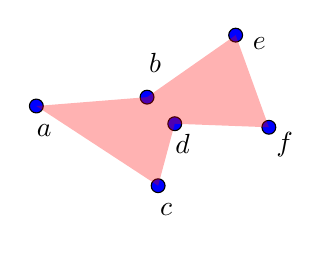
\begin{tikzpicture}[scale=.75]
            \node[draw, circle, black, fill=blue, inner sep=0pt, minimum size=5pt, label={[xshift=0.1cm, yshift=-0.6cm]$a$}] (a) at (1*2.5*0.75,6*0.4*0.75) {};
            \node[draw, circle, black, fill=blue, inner sep=0pt, minimum size=5pt, label={[xshift=0.1cm, yshift=0.1cm]$b$}] (b) at (2*2.5*0.75,6.5*0.4*0.75) {};
            \node[draw, circle, black, fill=blue, inner sep=0pt, minimum size=5pt, label={[xshift=0.1cm, yshift=-0.6cm]$c$}] (c) at (2.1*2.5*0.75,1.5*0.4*0.75) {};
            \node[draw, circle, black, fill=blue, inner sep=0pt, minimum size=5pt, label={[xshift=0.1cm, yshift=-0.6cm]$d$}] (d) at (2.25*2.5*0.75,5*0.4*0.75) {};
            \node[draw, circle, black, fill=blue, inner sep=0pt, minimum size=5pt, label={[xshift=0.3cm, yshift=-0.4cm]$e$}] (e) at (2.8*2.5*0.75,10*0.4*0.75) {};
            \node[draw, circle, black, fill=blue, inner sep=0pt, minimum size=5pt, label={[xshift=0.2cm, yshift=-0.6cm]$f$}] (f) at (3.1*2.5*0.75,4.8*0.4*0.75) {};
            \coordinate (a) at (1*2.5*0.75,6*0.4*0.75);
            \coordinate (b) at (2*2.5*0.75,6.5*0.4*0.75);
            \coordinate (c) at (2.1*2.5*0.75,1.5*0.4*0.75);
            \coordinate (d) at (2.25*2.5*0.75,5*0.4*0.75);
            \coordinate (e) at (2.8*2.5*0.75,10*0.4*0.75);
            \coordinate (f) at (3.1*2.5*0.75,4.8*0.4*0.75);
            \fill[red, opacity=0.3] (a) -- (b) -- (e) -- (f) -- (d) -- (c) -- (a) -- cycle;
        \end{tikzpicture}
        \caption{}\label{fig:equiv-c}
    \end{subfigure}
    \begin{subfigure}{0.24\linewidth}
        \centering
        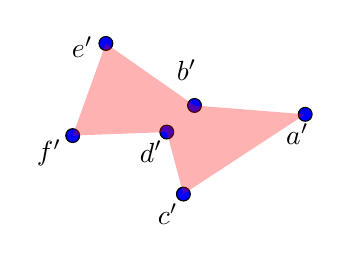
\begin{tikzpicture}[scale=.75]
            \node[draw, circle, black, fill=blue, inner sep=0pt, minimum size=5pt, label={[xshift=-0.1cm, yshift=-0.6cm]$a'$}] (a) at (-1*2.5*0.75,6*0.4*0.75) {};
            \node[draw, circle, black, fill=blue, inner sep=0pt, minimum size=5pt, label={[xshift=-0.1cm, yshift=0.1cm]$b'$}] (b) at (-2*2.5*0.75,6.5*0.4*0.75) {};
            \node[draw, circle, black, fill=blue, inner sep=0pt, minimum size=5pt, label={[xshift=-0.2cm, yshift=-0.6cm]$c'$}] (c) at (-2.1*2.5*0.75,1.5*0.4*0.75) {};
            \node[draw, circle, black, fill=blue, inner sep=0pt, minimum size=5pt, label={[xshift=-0.2cm, yshift=-0.6cm]$d'$}] (d) at (-2.25*2.5*0.75,5*0.4*0.75) {};
            \node[draw, circle, black, fill=blue, inner sep=0pt, minimum size=5pt, label={[xshift=-0.3cm, yshift=-0.4cm]$e'$}] (e) at (-2.8*2.5*0.75,10*0.4*0.75) {};
            \node[draw, circle, black, fill=blue, inner sep=0pt, minimum size=5pt, label={[xshift=-0.3cm, yshift=-0.6cm]$f'$}] (f) at (-3.1*2.5*0.75,4.8*0.4*0.75) {};
            \coordinate (a) at (-1*2.5*0.75,6*0.4*0.75);
            \coordinate (b) at (-2*2.5*0.75,6.5*0.4*0.75);
            \coordinate (c) at (-2.1*2.5*0.75,1.5*0.4*0.75);
            \coordinate (d) at (-2.25*2.5*0.75,5*0.4*0.75);
            \coordinate (e) at (-2.8*2.5*0.75,10*0.4*0.75);
            \coordinate (f) at (-3.1*2.5*0.75,4.8*0.4*0.75);
            \fill[red, opacity=0.3] (a) -- (b) -- (e) -- (f) -- (d) -- (c) -- (a) -- cycle;
        \end{tikzpicture}
        \caption{}\label{fig:equiv-d}
    \end{subfigure}
  \caption{The pointsets depicted in \Cref{fig:equiv-a,fig:equiv-b} do not require the parity option to be shown $\sigma$-equivalent, since the bijection $f$ defined by $(a,b,c,d) \mapsto (b', d', c', a')$ already satisfies $\sigma(p_i, p_j, p_k) = \sigma(f(p_i), f(p_j), f(p_j))$ for every $\{p_i, p_j, p_k\} \subseteq \{a,b,c,d\}.$ On the other hand, no such bijection exists for~\Cref{fig:equiv-c,fig:equiv-d},  which require the parity option for $\sigma$-equivalence. }\label{fig:sigma-equiv}
  %We obtained~\Cref{fig:equiv-c,fig:equiv-d} computationally.
  \end{figure}
